\section{Geometria de Uma e Duas Câmeras}

\subsection{Notação Básica de Geometria Projetiva}

Nesta seção, faremos uma breve introdução aos conceitos básicos de Geometria Projetiva e usaremos a notação contida em \cite{Hartley2004}, por ser o tipo de notação mais difundido entre pesquisas de visão computacional. Para uma abordagem mais profunda do assunto o leitor pode pesquisar o referido autor.  

\subsubsection{O Espaço Projetivo em Duas Dimensões}



\noindent {\bf A Reta}


Sabemos que uma reta no plano $\mathbb{R}^{2}$ pode ser representada pela equação $a\,x+b\,y+c=0$, onde a reta fica perfeitamente determinada pelos valores das constantes $a,b,c$. Desta forma, podemos representar retas através de vetores, e assim a reta $a\,x+b\,y+c=0$ seria representada por $(a,b,c)^\top \in \mathbb{R}^{3}$, utlizando o símbolo em negrito $\lightrgb$ para indicar tal vetor escrito em coluna, por padrão. Portanto $\lightrgb = (a,b,c)^\top$. Note que a relação entre uma dada reta e o seu respectivo vetor não é biunívoca, pois o vetor $k\,(a,b,c)^\top$, tal que $k \in \mathbb{R}$, representa a reta $k\,a\,x+k\,b\,y+k\,c=0$ que é a mesma reta $a\,x+b\,y+c=0$. Temos, então, infinitos vetores (chamados paralelos na Álgebra Linear) que representam uma mesma reta e formam uma classe de equivalência, onde essa classe pode ser representada por qualquer um de seus vetores. Os vetores de uma classe de equivalência, definida pela multiplicação por um escalar, são conhecidos como vetores {\it homogêneos}. O conjunto de classes de equivalência de vetores em $\mathbb{R}^{3} - (0,0,0)^\top$ forma o {\it Espaço Projetivo} $\mathbb{P}^{2}$. O vetor $(0,0,0)^\top$ foi excluído por não representar reta alguma. Após essas considerações, dizemos que uma reta no plano é representada pelo vetor $(a,b,c)^\top$ em {\it coordenadas homogêneas}. Já que para determinar uma reta precisamos determinar os valores do três parâmetros $a,b \,\,\text{e}\,\, c$, vemos que uma reta tem três graus de liberdade.\\

\noindent {\bf O Ponto}


Sabemos que em $\mathbb{R}^{2}$ os pontos são representados através de pares ordenados do tipo $(x,y)$, e assim cada ponto pode ser identificado como um vetor $(x,y)^\top$. Os vetores que se referem a pontos serão representados pelo símbolo em negrito $\x$, que sempre indicará um vetor coluna. Desse jeito, $\x=(x,y)^\top$. Sabemos também que um ponto $(x,y)^\top$ pertence a uma reta $(a,b,c)^\top$ se, e somente se, $a\,x+b\,y+c=0$, e podemos realizar essa verificação utilizando multiplicação matricial, escrevendo $\x$ com uma terceira coordenada igual a 1:

\begin{center}
$\begin{array}{ccccc}
 (x,y,1)^\top 
&\begin{pmatrix}
 a  \\ 
 b  \\ 
 c 
 \end{pmatrix} 
& = 0 \qquad 
& \text{ou} 
& \qquad \x ^T\lightrgb = 0.
\end{array}$
\end{center}

Ou seja, temos um ponto de $\mathbb{R}^{2}$ representado como um vetor com três coordenadas. Observe que para $k \in \mathbb{R} - \{0\}$, temos:

\begin{center}
$\begin{array}{ccccccc}
 (k\,x,k\,y,k)^\top 
&\begin{pmatrix}
 a  \\ 
 b  \\ 
 c 
 \end{pmatrix} 
& = 0
& \qquad \Leftrightarrow \qquad
& (x,y,1)^\top
&\begin{pmatrix}
 a  \\ 
 b  \\ 
 c 
 \end{pmatrix} 
& = 0.
\end{array}$
\end{center}

Portanto,  variando $k$, podemos considerar os vetores em coordenadas homogeneas $(k\,x,k\,y,k)^\top \in \mathbb{P}^2$, como representantes do mesmo ponto $(x,y)^\top \in \mathbb{R}^2$, e podemos resgatar nossa representaçao original aplicando o procedimento $(x/k,y/k)^\top$, pois $k \ne 0$.

\begin{figure}[!htb]
\centering
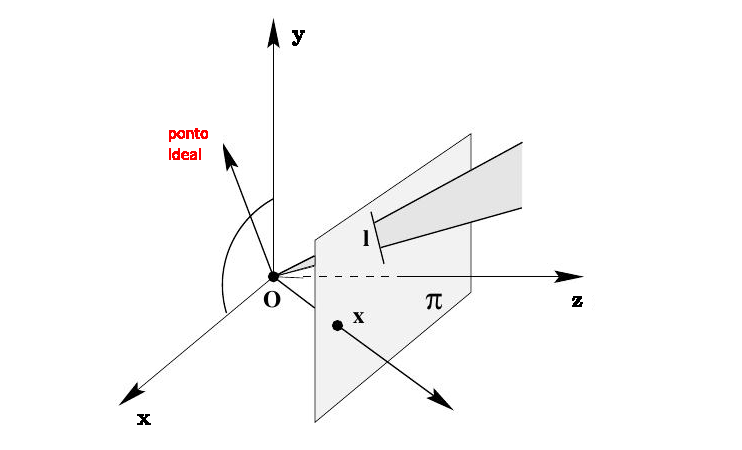
\includegraphics[scale=0.8]{espaco_P2}
\caption{\textit{O plano $\pi$ representa o espaço projetivo $\mathbb{P}^2$. Pontos e retas pertencentes a esse espaço são representados, respectivamente, por raios e planos que passam pela origem do $\mathbb{R}^3$.}}
\label{plano_P2}
\end{figure}

Podemos pensar no espaço projetivo como um conjunto de raios passando pela origem do $\mathbb{R}^3$, onde cada raio representa um único ponto, que é a interseção desse raio com o plano $\mathbb{P}^2$. Desta mesma forma, retas em $\mathbb{P}^2$ são formadas por planos. Na figura \ref{plano_P2}, podemos observar como a interseção do raio com o plano define um ponto, assim como a interseção de dois planos definem uma reta.


Para determinar um ponto precisamos determinar os valores das duas primeiras coordenadas do vetor homogêneo que representa esse ponto, já que a terceira coordenada está em função das duas primeiras. Assim, dizemos que um ponto tem dois graus de liberdade e a terceira coordenada pode ser usada para fixar uma escala.
\\

\noindent {\bf A Cônica}


Em geometria Euclidiana, as cônicas são de três tipos principais: elipse, hipérbole e parábola. São definidas, algebricamente, por uma equação do segundo grau em duas variáveis, considerando coordenadas não homogêneas:

\begin{equation*}
a\,x^2+b\,x\,y+c\,y^2+d\,x+e\,y+f=0.
\end{equation*}

Sabemos que um ponto pertence à cônica se ele é solução da equação acima, a qual pode ser representada utilizando multiplicação matricial e vetores em coordenadas homogêneas, com a terceira coordenada configurada como 1:

\begin{center}
$
\begin{array}{cccc}
  (x,y,1)^\top 
& \begin{bmatrix}
a & b/2 & d/2\\
b/2 & c & e/2\\
d/2 & e/2 & f
\end{bmatrix}
& \begin{pmatrix}
x\\
y\\
1
\end{pmatrix}
& = 0.
\end{array}
$
\end{center}

Podemos generalizar essas coordenadas homogêneas fazendo as substituições $x = x_{1}/x_{3}$ e $y = x_{2}/x_{3}$, e nossa equação do elípse fica:

\begin{equation*}
a\,x_1^2+b\,x_1\,x_2+c\,x_2^2+d\,x_1\,x_3+e\,x_2\,x_3+f\,x_3^2=0.
\end{equation*}

Novamente em notação matricial:

\begin{center}
$
\begin{array}{cccccc}
  (x_1,x_2,x_3)^\top 
& \begin{bmatrix}
  a & b/2 & d/2\\
  b/2 & c & e/2\\
  d/2 & e/2 & f
  \end{bmatrix}
& \begin{pmatrix}
  x_1\\
  x_2\\
  x_3
  \end{pmatrix}
& = 0
& \qquad \text{ou} \qquad
& \x^\top\,C\,\x = 0.
\end{array}
$
\end{center}

Já que um ponto pertence à cônica se, e somente se, satisfaz a última equação, temos que $C$ fica definida como a matriz que representa uma cônica no espaço projetivo $\mathbb{P}^2$.

\begin{center}
$
\begin{array}{cc}
C = & \begin{bmatrix}
      a & b/2 & d/2\\
      b/2 & c & e/2\\
      d/2 & e/2 & f
      \end{bmatrix}.
\end{array}
$
\end{center}


Percebemos que as cônicas são representadas por matrizes $3\times3$ simétricas e, portanto, possuem seis variáveis. Usando uma dessas variáveis para fixar a escala, temos que as cônicas possuem cinco graus de liberdade. Podemos, por exemplo, dividir todas as coordenadas da matriz $C$ por $f$. 

\subsubsection{O Espaço Projetivo em Três Dimensões}


\noindent {\bf O Ponto}


Analogamente à representação de um ponto no espaço $\mathbb{P}^2$, um ponto no espaço $\mathbb{P}^3$ é repesentado através de coordenadas homogêneas, acrescentando-se uma quarta coordenada ao vetor que representa esse ponto. Desta forma, $\X = (X_1,X_2,X_3,X_4)^\top$ e $X_4 \ne 0$, onde $\X$ é a representação em coordenadas homogêneas do ponto $(X,Y,Z)^\top \in \mathbb{R}^3$. Portanto esse vetor continua tendo três graus de liberdade. Para realizar tal mudança basta tomar 

\begin{equation*}
X=X_1/X_4 \,\, ,\, Y=X_2/X_4 \,\,\, \text{e} \,\,\, Z=X_3/X_4.
\end{equation*}

 

\noindent {\bf O Plano}

Temos que a representação algébrica de um plano $\bpi$ no espaço $\mathbb{R}^3$ é dada pela equação

\begin{equation*}
\pi_1\,X+\pi_2\,Y+\pi_3\,Z+\pi_4=0,
\end{equation*}
onde $\pi_i$ são os coeficientes da equação.

Um ponto em $\mathbb{R}^3$ pertence ao plano se, e somente se, satifaz a equação acima que na forma matricial usando a representação do ponto em coordenadas homogêneas fica:

\begin{center}
$
\begin{array}{ccc}
  (\pi_1,\pi_2,\pi_3,\pi_4)^\top
& \begin{pmatrix}
  X\\
  Y\\
  Z\\
  1
  \end{pmatrix}
& = 0.
\end{array}
$
\end{center}

Fazendo as substituições 
\begin{equation*}
X=X_1/X_4 \,\, , \,\, Y=X_2/X_4 \,\,\,\, \text{e} \,\,\,\, Z=X_3/X_4 ,
\end{equation*}

generalizamos a representação do ponto e a equação se torna:

\begin{center}
$
\begin{array}{ccccc}
(\pi_1,\pi_2,\pi_3,\pi_4)^\top
& \begin{pmatrix}
  X_1\\
  X_2\\
  X_3\\
  X_4
  \end{pmatrix}
& = 0
& \qquad \text{ou} \qquad
& \bpi^\top \, \X = 0.
\end{array}
$
\end{center}


Desta forma, verificamos que, assim como os pontos, um plano $\bpi = (\pi_1,\pi_2,\pi_3,\pi_4)^\top$ fica inteiramente determinado por um vetor com quatro coordenadas em $\mathbb{P}^3$. Aqui temos uma analogia com o espaço $\mathbb{P}^2$, já que pontos e retas têm a mesma representação vetorial com três coordenadas naquele espaço. Como multiplicar a equação algébrica de um plano por um escalar diferente de zero não altera seu valor, temos que os planos possuem três graus de liberdade. Podemos dividir as três primeiras coordenadas pela última, por exemplo, e fixar um escala.

Obs: As três primeiras coordenadas do vetor que representa o plano corresponde ao vetor normal ao plano, conforme definido em Álgebra Linear.
\\


\noindent {\bf A Reta}

Uma reta pode ser definida passando por dois pontos. Em $\mathbb{P}^2$, como os dois pontos estão no mesmo plano, uma reta passando por esses dois pontos tem apenas três graus de liberdade, conforme visto anteriormente. Mas em $\mathbb{P}^3$, como os dois pontos podem estar em planos diferentes, temos que uma reta apresenta quatro graus de liberdade, dois graus para cada ponto. Assim, uma reta deveria ser representada por um vetor com cinco coordenadas em $\mathbb{P}^3$, mas vetores desse tipo não podem ser usados, facilmente, em expressões matemáticas que envolvem vetores com quatro coordenadas representando pontos e planos. Portanto é necessário encontrar uma outra representação, e uma das formas mais simples é definir a reta através de dois pontos não coincidentes. Outras representações de uma reta no espaço projetivo $\mathbb{P}^3$, diferentes da apresentada aqui, podem ser encontradas em \cite{Hartley2004}.


Uma reta ${\bf L}$ passando por dois pontos ${\bf A} \,\,\, \text{e} \,\,\, {\bf B}$ é representada pelo espaço linha gerado pela matriz $W$ composta pelos pontos ${\bf A}^\top \,\,\,\text{e} \,\,\, {\bf B}^\top$ em linha:

\begin{center}
$
\begin{array}{cc}
W = 
& \begin{bmatrix}
  A^\top\\
  B^\top
  \end{bmatrix},
\end{array}
$
\end{center}
onde os espaço gerado por $W^\top$ é o conjunto de pontos do tipo $a\,{\bf A} + b\,{\bf B}$ pertencentes à reta ${\bf L}$ procurada. \\


\noindent {\bf A Quádrica}


Similarmente à cônica em $\mathbb{P}^2$, uma quádrica $Q$ em $\mathbb{P}^3$ é definida pela equação

\begin{equation*}
\X^\top\,Q\,\X = 0,
\end{equation*}
onde $Q$ é uma matriz simétrica $4\times4$ com nove graus de liberdade.




\begin{figure}[!htb]
$
\begin{array}{cc}
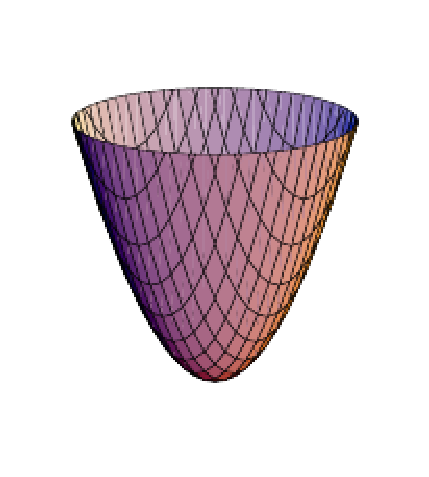
\includegraphics[scale=1.1]{paraboloide}
&
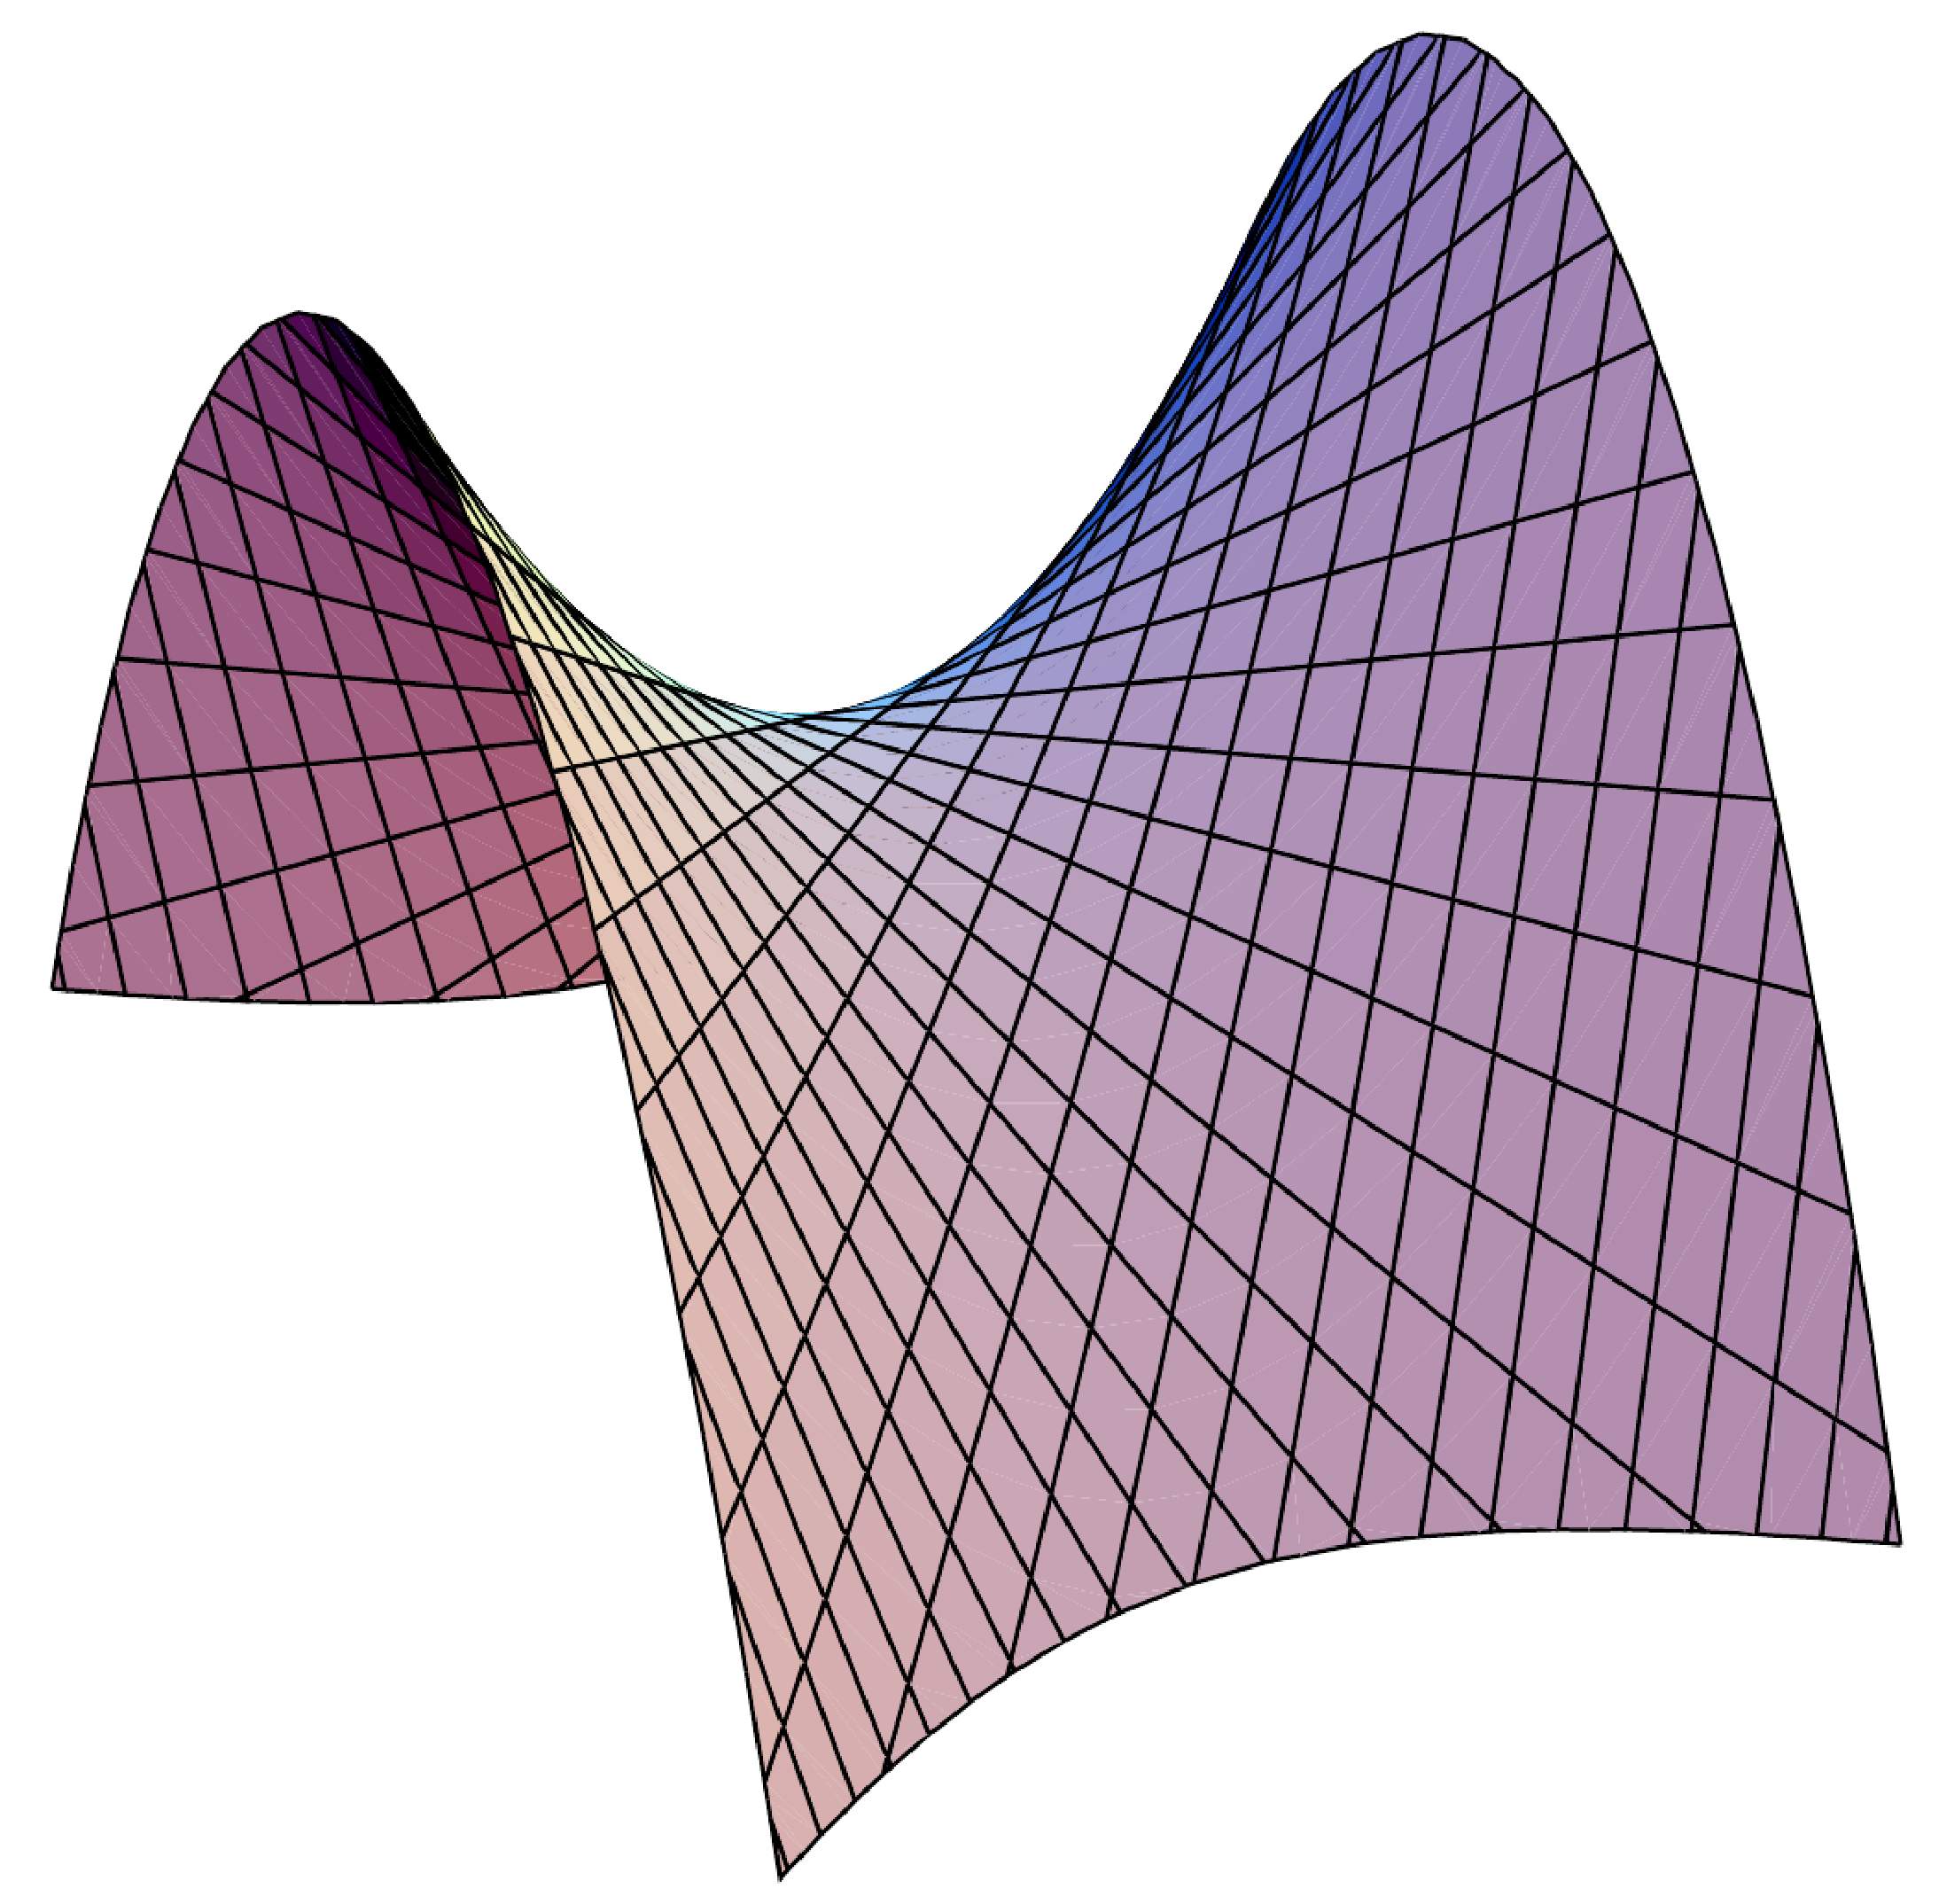
\includegraphics[scale=0.9]{hiperboloide_1_folha}
\end{array}
$
\caption{\textit{Parabolóide à esquerda e hiperbolóide de uma folha à direita.}}
\label{quadricas}
\end{figure}


Mais detalhes sobre a dedução da definição de uma quádrica podem ser encontrados em \cite{Hartley2004}, bem como outros exemplos além daqueles observados na figura \ref{quadricas}.

\subsubsection{A Câmera P}

A \textit{câmera} é uma transformação linear entre um ponto 3D no espaço e um ponto 2D no plano da imagem, representada por uma matriz com algumas propriedades que realizam o mapeamento entre os pontos. Existem vários tipos de câmera, mas para tratar das características básicas vamos utilizar o modelo buraco de alfinete, do inglês \textit{pinhole}.

Consideramos o \textit{centro de projeção}, ou \textit{centro da câmera}, como a origem do espaço tridimensional Euclidiano, com o \textit{plano da imagem} ou \textit{plano focal} sendo $Z = f$, onde $f$ é a \textit{distancia focal} entre o plano da imagem e o centro de projeção. Como podemos obeservar na figura \ref{camera}, um ponto $\X$ no espaço 3D é mapeado a um ponto $\x$ no plano da imagem por uma reta que liga $\X$ ao centro de projeção, e intersepta o plano da imagem. Assim, ignorando a última coordenada homogênea do vetor que representa o ponto na imagem, temos o mapeamento:

\begin{center}
$\X = (X,Y,Z)^\top \rightarrow \x = (fX/Z,fY/Z,f) \rightarrow (fX/Z,fY/Z)$  
\end{center}

O plano que passa pelo centro da câmera e é paralelo ao plano da imagem é chamado \textit{plano principal}, o plano $xy$ na figura \ref{camera}. O \textit{eixo principal} passa pelo centro da câmera e é perpendicular ao plano da imagem, onde a interseção desse eixo com o plano da imagem forma o \textit{ponto principal}.


\begin{figure}[!htb]
\centering
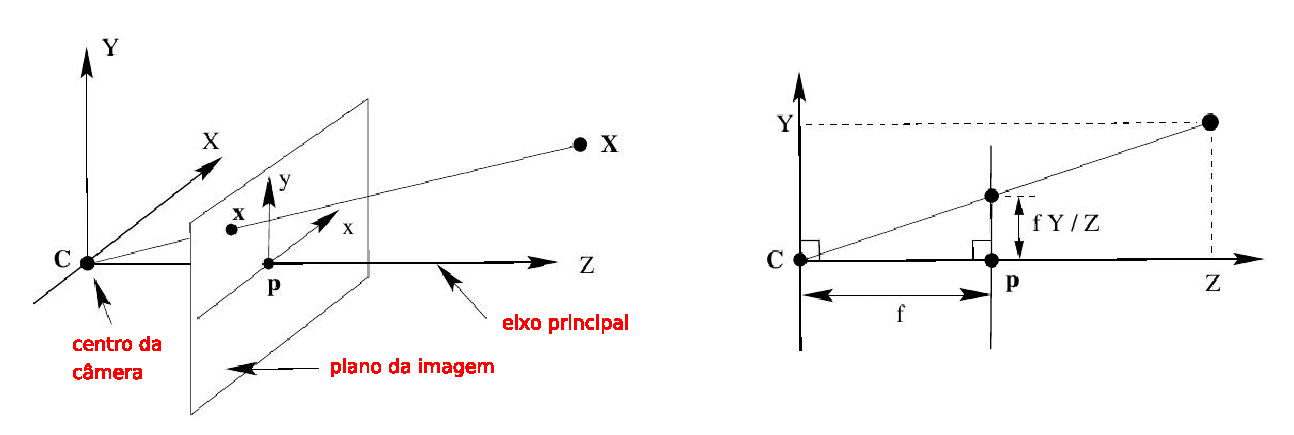
\includegraphics[scale=.64]{modelo_camera}
\caption{\textit{Visualização das características básicas de uma câmera como distância focal, eixo principal, plano da imagem, centro de projeção e o ponto principal {\bf P}.}}
\label{camera}
\end{figure}

Com vetores representados em coordenadas homogêneas, podemos expressar o mapeamento através de um operador linear, onde realizamos a multiplicação da matriz $P$, que representa a câmera, por um ponto no espaço, resultando num ponto na imagem conforme o esquema abaixo:

\begin{center}
$
\begin{array}{ccc}
\begin{pmatrix}
fX\\
fY\\
Z
\end{pmatrix} = 
&
\begin{bmatrix}
f& & &0\\
 &f& &0\\
 & &1&0
\end{bmatrix}
&
\begin{pmatrix}
X\\
Y\\
Z\\
1
\end{pmatrix}
\end{array}
$
\end{center}

Nessa matriz temos que $f$ é a distância focal (entre o centro da câmera e o plano da imagem), e o vetor de coluna de zeros à direita representa as coordenadas do centro da câmera, que nesse caso está na origem do sistema. Essa matriz pode ser desmembrada da seguinte maneria: uma matriz diagonal $diag(f,f,1)$ multiplicada pela matriz $[I|{\bf 0}]$, onde $I$ é uma matriz identidade $3\times3$ e ${\bf 0}$ é um vetor coluna de zeros. Compactamente, podemos escrever a ultima relaçao como:

\begin{center}
$\x = diag(f,f,1)\,[I|{\bf 0}]\,\X$,
\end{center}
onde $diag(f,f,1)\,[I|{\bf 0}]$ é a matriz da câmera para o modelo \textit{pinhole}.

Nessa dedução, consideramos que o ponto principal  coincide com a origem do plano da imagem, mas na prática isso pode não acontecer. Dessa forma, devemos acrescentar as coordenadas do ponto na construção da matriz da câmera. Sendo $(p_x,p_y)$ as coordenadas do ponto principal, desejamos o seguinte mapeamento:

\begin{center}
$(X,Y,Z)^\top \rightarrow (\frac{f\,X}{Z}+p_x\,,\,\frac{f\,Y}{Z}+p_y)$,
\end{center}
o qual nos fornece a seguinte relação de projeção em coordenadas homogêneas:

\begin{center}
$
\begin{array}{ccc}
\begin{pmatrix}
f\,X + Z\,p_x\\
f\,Y + Z\,p_y\\
Z
\end{pmatrix}=
&
\begin{bmatrix}
f& &p_x&0\\
 &f&p_y&0\\
 & &1&0
\end{bmatrix}
\begin{pmatrix}
X\\
Y\\
Z\\
1
\end{pmatrix}
\end{array}
$
\end{center}

Definindo a notação

\begin{center}
$
\begin{array}{cc}
K = & \begin{bmatrix}
      f& &p_x\\
       &f&p_y\\
       & &1
      \end{bmatrix}, 
\end{array}
$
\end{center}
a relação de projeção assume a forma


\begin{equation}
\x=K\,[I|{\bf 0}]\,\X_{\textit{cam}},
\end{equation}
onde $K$ é denominada matriz de calibração da câmera, a qual resume os parâmetros internos da mesma, e $\X_{\textit{cam}}$ enfatiza que o ponto 3D está escrito no sistema de coordenadas da câmera.

Até aqui temos expressado o ponto $\X$ no espaço em relação às coordenadas da câmera, assumindo que o centro da câmera está situado na origem do sistema de eixos, o qual recebe o nome de sistema de coordenadas da câmera. Mas na maioria das vezes esse não é o caso, portanto desejamos fazer o mapeamento de um ponto 3D cujo as coordenadas estejam expressas com relação a um sistema de coordenadas qualquer, chamado sistema de coordenadas do mundo. Portanto, vamos continuar completando a matriz $P$ para mapear pontos no sistema de coordenadas do mundo.

Considerando o sistema de coordenadas do mundo, denotaremos um ponto nesse sistema, em coordenadas não homogêneas, por $\overline{\X}$, e o mesmo ponto no sistema de coordenadas da câmera será denotado por $\overline{\X}_{\textit{cam}}$. A transferência de sistemas de coordenadas é feita através da relação $\overline{\X}_{\textit{cam}}=R\,(\overline{\X}-\overline{\bf C})$, onde $\overline{\bf C}$ representa o centro da câmera no sistema de coordenadas do mundo e $R$ representa uma matriz de rotação $3\times3$. Passando os vetores para coordenadas homogêneas, podemos aplicar a rotação no vetor $\overline{\bf C}$, do centro da câmera, e inseri-lo na quarta coluna da matriz escrevendo a relação

\begin{center}
$
\begin{array}{ccc}
\overline{\X}_{\textit{cam}}=
&
\begin{bmatrix}
R&-R\,\overline{\bf C}\\
\,\,{\bf 0}^\top&\,\,1
\end{bmatrix}
&
\begin{pmatrix}
X\\
Y\\
Z\\
1
\end{pmatrix},
\end{array}
$
\end{center} 
onde podemos escrever

\begin{center}
$
\begin{array}{cccc}
R=
&
\begin{bmatrix}
a&b&c\\
d&e&f\\
g&h&i
\end{bmatrix}
&
\qquad\text{e}\qquad
&
-R\,\overline{\bf C}=(t_1,t_2,t_3)^\top,
\end{array}
$
\end{center}
e a relação acima fica:

\begin{center}
$
\begin{array}{ccc}
\overline{\X}_{\textit{cam}}=
&
\begin{bmatrix}
a&b&c&t_1\\
d&e&f&t_2\\
g&h&i&t_3\\
0&0&0&\,1
\end{bmatrix}
&
\begin{pmatrix}
X\\
Y\\
Z\\
1
\end{pmatrix}.
\end{array}
$
\end{center}

Substituindo $\overline{\X}_{\textit{cam}}$ em (1), obtemos

\begin{center}
$
\begin{array}{ccccc}
\x=
&
\begin{bmatrix}
      f& &p_x\\
       &f&p_y\\
       & &1
\end{bmatrix}
&
\begin{bmatrix}
1&0&0&0\\
0&1&0&0\\
0&0&1&0
\end{bmatrix}
&
\begin{bmatrix}
a&b&c&t_1\\
d&e&f&t_2\\
g&h&i&t_3\\
0&0&0&\,1
\end{bmatrix}
&
\begin{pmatrix}
X\\
Y\\
Z\\
1
\end{pmatrix},
\end{array}
$
\end{center}
multiplicando a segunda e terceira matrizes,
 
\begin{center}
$
\begin{array}{cccc}
\x=
&
\begin{bmatrix}
      f& &p_x\\
       &f&p_y\\
       & &1
\end{bmatrix}
&
\begin{bmatrix}
a&b&c&t_1\\
d&e&f&t_2\\
g&h&i&t_3
\end{bmatrix}
&
\begin{pmatrix}
X\\
Y\\
Z\\
1
\end{pmatrix},
\end{array}
$
\end{center}
que pode ser escrita de forma resumida como

\begin{center}
$
\x=K\,[R|{\bf t}]\,\X,
$
\end{center}
com ${\bf t}=(t_1,t_2,t_3)^\top$ denominado vetor de translação.

Acabamos de incluir todos os parâmetros na matriz $P=K\,[R|{\bf t}]$, para o mapeamento de um ponto 3D homogêneo no sistema de coordenadas do mundo em seu respectivo ponto 2D no plano da imagem, no sistema de coordenadas da câmera. Temos três parâmetros internos na matriz de calibração $K$, $(f,p_x,p_y)$, três parâmetros externos na matriz de rotação $R$, apesar de suas nove entradas, e mais três parâmetros externos no vetor de translação. 


\subsection{Notação Usada por Fabbri}

Na seção anterior expusemos um tipo de notação bastante difundida na área de visão computacional mas que, por usar letras do nosso alfabeto, pode ocasionar alguma confusão ou mal entendido. Sendo assim, faz-se necessária a inclusão de uma nova notação que evite alguma ambiguidade e que favoreça a lucidez. Na tabela \ref{tab_not} temos um resumo da notação encontrada em \cite{Fabbri:Kimia:IJCV2015}, artigo o qual o leitor poderá consultar caso necessite de outras notações que não constam aqui. Essa nova notação é muito útil para a aplicação da projeção, já que para projetar um ponto na imagem fazemos a divisão de todas as três coordenadas desse ponto pela terceira coordenada. Outra ajuda acontece nas diferenciações, na obtenção das equações diferenciais e algébricas envolvidas no uso da geometria diferencial para abordar problemas do tipo. Nas abordagens feitas por hartley, usa-se correspondência de pontos e retas, basicamente, o que é feito pela maioria dos pesquisadores em visão computacional, e fica ruim para trabalhar com tangentes por conta dessa abordagem mais matricial. Com a notação apresentada aqui, as equações são explícitas e proporciona o emprego das tangentes.

\begin{table}[!h]
\begin{center}
\begin{tabular}{|c|l|}
\hline
Símbolos&Descrição\\\hline\hline
$\Gama^w$&Ponto 3D no sistema de coordenadas do mundo.\\\hline
$\Gama$&Ponto 3D no sistema de coordenadas da câmera.\\\hline
$\rot$&Matriz de rotação: coordenadas do mundo para a câmera.\\\hline
$\transl$&Vetor de translação.\\\hline
$\mathcal K$&Matriz de calibração: modelo basico (\textit{pinhole}).\\\hline
$\mathcal K_{im}$&Matriz de calibração: coordenadas do plano medidas em pixels.\\\hline
$\bc$&O centro da câmera.\\\hline
$\depth$&Profundidade do ponto imagem.\\\hline
$\gama$&Ponto 2D em coordenadas normalizadas.\\\hline
&Imagem da tangente a uma curva.\\\hline
$\T$&Tangente a uma curva no espaço: coordenadas da câmera.\\\hline
$\T^w$&Tangente a uma curva no espaço: coordenadas do mundo\\\hline
$K$&Curvatura.\\\hline
$G$&Velocidade de parametrizaçao.\\\hline
$\N^w$&Vetor normal.\\\hline
$\e_1$, $\e_2$, $\e_3$&Base de vetores do sistema de coordenadas da câmera.\\\hline
$\e_1^w$, $\e_2^w$, $\e_3^w$&Base de vetores do sistema de coordenadas do mundo.\\\hline
\end{tabular}
\end{center}
\caption{Notação.}
\label{tab_not}
\end{table}

Dada uma curva no espaço 3D conforme a figura \ref{curva_3D}, podemos fazer a representação de seus pontos nas coordenadas da câmera em função da representação dos mesmos pontos nas coordenadas do mundo de acordo com a relação:

\begin{figure}[!htb]
\centering
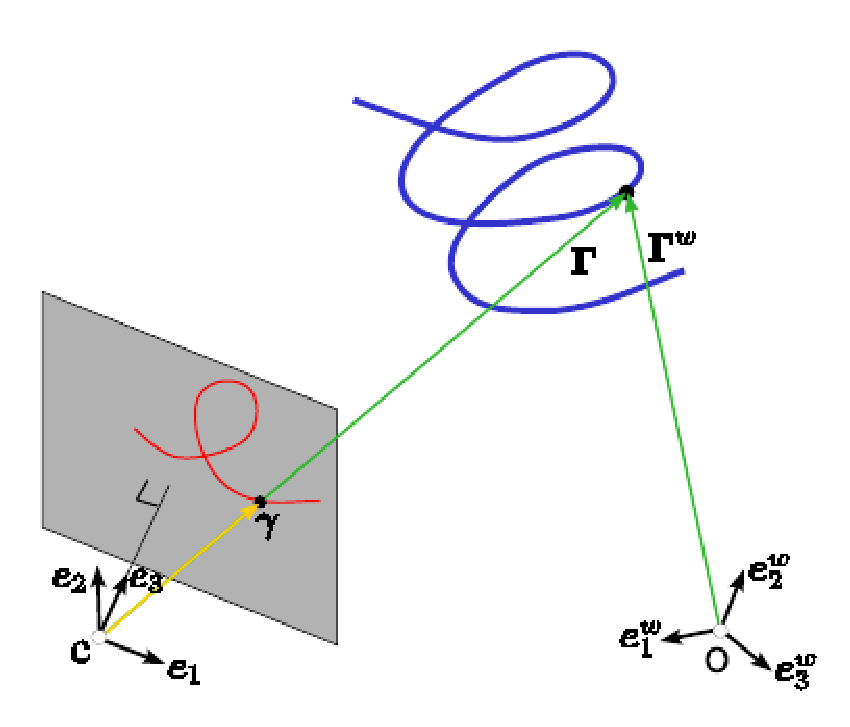
\includegraphics[scale=.8]{curva}
\caption{\textit{Cruva no espaço 3D e sua respectiva imagem 2D. Observe a representação de um mesmo ponto nas coordenadas do mundo e nas coordenadas da câmera.}}
\label{curva_3D}
\end{figure}


\begin{equation}\label{eq:coord:transf:RT}
\Gama = \rot (\Gama^w - \bc) \qquad \text{ou} \qquad \Gama = \rot\Gama^w + \transl,
\end{equation}
onde $\transl = -\rot\bc$ são as coordenadas da origem do espaço 3D expressas no sistema de coordenadas da câmera, e $\rot$ é a matriz de rotação.

A projeção de um ponto 3D $\Gama = [x,\, y,\, z]^\top$ no plano da imagem $z=1$ é o ponto $\gama = [\uu,\,\vv,\,1]^\top$ e esses pontos estão relacionados por:

\begin{equation}\label{eq:projection}[x,\, y,\, z]^\top =
[\depth\uu,\,\depth\vv,\,\depth]^\top \,\,\,\,\text{ou, compactamente,}\,\,\,\,  \Gama =
\depth\gama,
\end{equation}
onde $\depth$ é a profundidade extraída da terceira coordenada do vetor que representa o ponto 3D escrito nas coordenadas da câmera, $\depth = z = \e_3^\top\Gama$, e $\e_3^\top = [0,0,1]^\top$.

Substituindo $\depth$ em \ref{eq:projection} e isolando $\gama$, temos

\begin{align}
\gama &= \frac{\Gama}{\f^\top\Gama}.
\label{eq:projection:isolated:gamma}
\end{align}
e assim observamos que pontos na imagem são sempre tratados como um vetor 3D com $z=1$. 

Denotendo por $\gama^{(i)}$ a $i^{th}$ derivada de $\gama$ em relação a um parâmetro qualquer para $i$ um número natural, podemos verificar que

\begin{equation*}
\f^\top\gama^{(i)} = 0 \qquad \text{e} \qquad \f^\top\Gama^{(i)} = \depth^{(i)}.
\end{equation*}

Mais especificamente, calculando as derivadas primeira e segunda de $\depth$ obtemos

\begin{equation}\label{eq:depth:derivs}
\depth =
\e_3^\top\Gama,\qquad \depth' = G\e_3^\top\T,\qquad \depth'' = G'\e_3^\top\T +
G^2K\e_3^\top\N
\end{equation}
onde $G$ é a velocidade de parametrização, $\T^w$ é a tangente à curva no ponto $\Gama^{w}$ no espaço 3D, $K$ é a curvatura, e $\N^w$ é o vetor normal, cada qual com as seguintes definições:

\begin{equation}\label{eq:definicoes}
G  = \|\Gama^{w'}\|,\qquad \T^w = \frac{\Gama^{w'}}{G}, \qquad K  = \frac{\|\T^{w'}\|}{G} \qquad \text{e} \qquad \N^w = \frac{\T^{w'}}{\|\T^{w'}\|}.
\end{equation}

As definições da tangente e do vetor normal em \ref{eq:definicoes} foram dadas no sistema de coordenadas do mundo, enquanto em \ref{eq:depth:derivs} os mesmos são dados no sistema de coordenadas da câmera. Como visto anteriormente, para fazer a conversão basta aplicar 

\begin{equation*}
\T = \rot\T^w \qquad \text{e} \qquad \N = \rot\N^w,
\end{equation*}
e é interessante notar que para pontos perto/longe da curva temos $\depth' = 0$, $\e_3^\top\T = 0$.


Lembramos que a matriz de calibração para o modelo básico \textit{pinhole} é

\begin{center}
$
\begin{array}{cc}
\mathcal K = & \begin{bmatrix}
               f& &p_x\\
                &f&p_y\\
                & &1
               \end{bmatrix}, 
\end{array}
$
\end{center}
mas na prática, pontos na imagem são descritos em pixels, $\gama_{im} = [x_{im},\, y_{im},\, 1]^\top$ após a aplicação da matriz de calibração com os parâmetros internos 

\begin{equation}\label{eq:intrinsic:parameter:transf}
\gama_{im} = \mathcal K_{im}\gama,
\ \ \ \ \ \
\mathcal K_{im} = \begin{bmatrix}
\alpha_\uu & \sigma & \uu_o\\
0 &\alpha_\vv &  \vv_o\\
0 & 0 &  1
\end{bmatrix},
\end{equation}
onde $\uu_o$ e $\vv_o$ são as coordenadas do ponto principal na imagem, $\sigma$ define a inclinação entre os eixos cartesianos no plano da imagem (se $\sigma=0$ os eixos são perpendiculares), e
$\alpha_\uu$ e $\alpha_\vv$ são calculados dividindo-se a distância focal $f$ pela largura e altura do pixel medidas em unidades do mundo, respectivamente. Sendo $m_x$ e $m_y$ a largura e altura do pixel temos:

\begin{equation*}
\uu_o = \frac{p_x}{m_x}, \qquad \vv_o = \frac{p_y}{m_y}, \qquad \alpha_\uu = \frac{f}{m_x}, \qquad \alpha_\vv = \frac{f}{m_y}.
\end{equation*}


\subsection{Resumo dos Resultados Fabbri}
Projeção e reconstrução 3D com o uso de tangentes.

